
%(BEGIN_QUESTION)
% Copyright 2010, Tony R. Kuphaldt, released under the Creative Commons Attribution License (v 1.0)
% This means you may do almost anything with this work of mine, so long as you give me proper credit

The flow rate of liquid spilling over a {\it rectangular weir} may be calculated by the height of that liquid over the weir by the following formula:

$$\includegraphics[width=15.5cm]{i04543x01.eps}$$

A technician tries to program a PLC to evaluate this formula so that the PLC may continuously calculate flow rate from measured liquid height, but the PLC program keeps ``faulting'' due to its inability to handle fractional exponents (the ``1.5'' power in the formula).

\vskip 10pt

Find a way for the PLC to evaluate this equation using nothing but integer-value exponents.

\vfil
\underbar{file i04543}
\eject
%(END_QUESTION)





%(BEGIN_ANSWER)

This is a graded question -- no answers or hints given!

%(END_ANSWER)





%(BEGIN_NOTES)

PLC processors tend to be a lot more limited than general-purpose computers when it comes to doing arithmetic.  Many PLCs can only do math on the level of a simple hand calculator.  Such is the case here: the application demands that we calculate the 1.5 power of a variable, but unfortunately this particular PLC simply isn't capable of doing that kind of calculation.

\vskip 10pt

For a solution, therefore, we need to find some mathematical equivalent of the 1.5 power.  In other words, we need to find some way to do the same arithmetic using some other function(s).  One way to do this is to recall from basic algebra that fractional exponents are equivalent to roots (e.g. $x^{1 \over 2} = x^{0.5} = \sqrt{x}$).  We know that an exponent of 1.5 is equivalent to a fractional value of $3 \over 2$, which gives us a way to calculate the 1.5 power using cube ($x^3$) and square-root ($x^{1 \over 2}$) functions:

$$Q = 3.33 (L - 0.2H) H^{1.5}$$

$$Q = 3.33 (L - 0.2H) H^{3 \over 2}$$

$$Q = 3.33 (L - 0.2H) \sqrt{H^{3}}$$

Another mathematical ``trick'' useful for calculating odd powers is to use logarithms.  Recall from algebra that the logarithm of a number raised to a power is equal to that power multiplied by the logarithm of the number:

$$\log x^y = y \log x$$

Un-doing the logarithm function with an ``antilog'' function yields the original argument:

$$10^{\log x^y} = 10^{y \log x} = x^y$$

Another way to write this is to say ``antilog'' rather than to explicitly show an exponential function:

$$\hbox{antilog}(\log x^y) = \hbox{antilog}(y \log x) = x^y$$

It is common to find PLCs that cannot calculate fractional exponents, but which can calculate logarithms and anti-logarithms.  In this case, the logarithm-based solution would look like:

$$Q = 3.33 (L - 0.2H) [\hbox{antilog}(1.5 \log H)]$$

%INDEX% PLC, ladder logic programming: integer math limitations

%(END_NOTES)

